%%
%% This is file `sample-sigconf.tex',
%% generated with the docstrip utility.
%%
%% The original source files were:
%%
%% samples.dtx  (with options: `all,proceedings,bibtex,sigconf')
%% 
%% IMPORTANT NOTICE:
%% 
%% For the copyright see the source file.
%% 
%% Any modified versions of this file must be renamed
%% with new filenames distinct from sample-sigconf.tex.
%% 
%% For distribution of the original source see the terms
%% for copying and modification in the file samples.dtx.
%% 
%% This generated file may be distributed as long as the
%% original source files, as listed above, are part of the
%% same distribution. (The sources need not necessarily be
%% in the same archive or directory.)
%%
%%
%% Commands for TeXCount
%TC:macro \cite [option:text,text]
%TC:macro \citep [option:text,text]
%TC:macro \citet [option:text,text]
%TC:envir table 0 1
%TC:envir table* 0 1
%TC:envir tabular [ignore] word
%TC:envir displaymath 0 word
%TC:envir math 0 word
%TC:envir comment 0 0
%%
%% The first command in your LaTeX source must be the \documentclass
%% command.
%%
%% For submission and review of your manuscript please change the
%% command to \documentclass[manuscript, screen, review]{acmart}.
%%
%% When submitting camera ready or to TAPS, please change the command
%% to \documentclass[sigconf]{acmart} or whichever template is required
%% for your publication.
%%
%%
\documentclass[sigconf,nonacm]{acmart}
%%
%% \BibTeX command to typeset BibTeX logo in the docs
\AtBeginDocument{%
  \providecommand\BibTeX{{%
    Bib\TeX}}}

%% Rights management information.  This information is sent to you
%% when you complete the rights form.  These commands have SAMPLE
%% values in them; it is your responsibility as an author to replace
%% the commands and values with those provided to you when you
%% complete the rights form.
\setcopyright{acmlicensed}
\copyrightyear{2018}
\acmYear{2018}
\acmDOI{XXXXXXX.XXXXXXX}
%% These commands are for a PROCEEDINGS abstract or paper.
\acmConference[Conference acronym 'XX]{Make sure to enter the correct
  conference title from your rights confirmation email}{June 03--05,
  2018}{Woodstock, NY}
%%
%%  Uncomment \acmBooktitle if the title of the proceedings is different
%%  from ``Proceedings of ...''!
%%
%%\acmBooktitle{Woodstock '18: ACM Symposium on Neural Gaze Detection,
%%  June 03--05, 2018, Woodstock, NY}
\acmISBN{978-1-4503-XXXX-X/2018/06}


%%
%% Submission ID.
%% Use this when submitting an article to a sponsored event. You'll
%% receive a unique submission ID from the organizers
%% of the event, and this ID should be used as the parameter to this command.
%%\acmSubmissionID{123-A56-BU3}

%%
%% For managing citations, it is recommended to use bibliography
%% files in BibTeX format.
%%
%% You can then either use BibTeX with the ACM-Reference-Format style,
%% or BibLaTeX with the acmnumeric or acmauthoryear sytles, that include
%% support for advanced citation of software artefact from the
%% biblatex-software package, also separately available on CTAN.
%%
%% Look at the sample-*-biblatex.tex files for templates showcasing
%% the biblatex styles.
%%

%%
%% The majority of ACM publications use numbered citations and
%% references.  The command \citestyle{authoryear} switches to the
%% "author year" style.
%%
%% If you are preparing content for an event
%% sponsored by ACM SIGGRAPH, you must use the "author year" style of
%% citations and references.
%% Uncommenting
%% the next command will enable that style.
%%\citestyle{acmauthoryear}


%%
%% end of the preamble, start of the body of the document source.
% This template file contains packages and commands that are useful and generic
% across papers.
%
% When adding new commands, you can most likely do that within paper.tex, but
% when adding new packages, you might need to update that here to ensure the
% packages are included in the proper order (a common source of compilation
% errors with LaTeX).

%%%%%%%%%%%%%%%%%%%%%%%%%%%%%%%%%%%%%%%%%%%%%%%%%%%%%%%%%%%%%%%%%%%%%%%%%%%%
% Packages {{{

\usepackage{color}
\usepackage{graphicx}
\usepackage[labelformat=simple]{subcaption}
%%\usepackage{wrapfig}
\usepackage{xspace}
\usepackage{multirow}
\usepackage{makecell} % Not sure if we need this
% see: https://tex.stackexchange.com/questions/170772/command-labelindent-already-defined
%\let\labelindent\relax
\usepackage{enumitem}

\usepackage[ruled,vlined]{algorithm2e}

\usepackage{ulem}
\normalem

\usepackage{tikz}
\newcommand*\circled[1]{\tikz[baseline=(char.base)]{
            \node[shape=circle,fill,inner sep=1.8pt] (char) {\small\textcolor{white}{#1}};}}
\newcommand*\wcircled[1]{\tikz[baseline=(char.base)]{
            \node[shape=circle,draw,inner sep=1.8pt] (char) {\small #1};}}

\usepackage{tcolorbox}
\usepackage{listings}

% }}}
%%%%%%%%%%%%%%%%%%%%%%%%%%%%%%%%%%%%%%%%%%%%%%%%%%%%%%%%%%%%%%%%%%%%%%%%%%%%
% Commands {{{

\newcommand{\etal}{et~al.\xspace}

\newcommand{\cmark}{\ding{51}}%
\newcommand{\xmark}{\ding{55}}%

\renewcommand\thesubfigure{(\alph{subfigure}) }

\newcommand{\parhead}[1]{\medskip \noindent \textbf{#1}\hskip .1in}


% }}}
%%%%%%%%%%%%%%%%%%%%%%%%%%%%%%%%%%%%%%%%%%%%%%%%%%%%%%%%%%%%%%%%%%%%%%%%%%%%
% Environments {{{

\newenvironment{strategy}[1][htb]
  {\renewcommand{\algorithmcfname}{Strategy}
   \begin{algorithm}[#1]%
  }{
   \end{algorithm}
   }
  
\newenvironment{tightlist}{
	\begin{list}{$\bullet$} {
		\setlength{\itemsep}{0.00cm}
		\setlength{\parskip}{-0.1cm} 
	}}{\end{list}}

\newenvironment{widelist}{
	\begin{list}{$\bullet$} {
		\setlength{\leftmargin}{.70cm}
		\setlength{\itemsep}{.00cm}
	}}{\end{list}}

% }}}
%%%%%%%%%%%%%%%%%%%%%%%%%%%%%%%%%%%%%%%%%%%%%%%%%%%%%%%%%%%%%%%%%%%%%%%%%%%%
% Comment Commands {{{

\ifdefined\isFinalized
\newcommand{\NewCommentType}[3]{}
\else
\newcommand{\NewCommentType}[3]{\expandafter\newcommand\csname #1\endcsname[1]{{\color{#2}{#3: ##1}} }}
\fi

% }}}
%%%%%%%%%%%%%%%%%%%%%%%%%%%%%%%%%%%%%%%%%%%%%%%%%%%%%%%%%%%%%%%%%%%%%%%%%%%%
% Line-break nudging {{{

\clubpenalty=10000 
\widowpenalty = 10000 

\hyphenation{de-a-non-y-mi-za-tion}
\hyphenation{none-the-less}

% }}}
%%%%%%%%%%%%%%%%%%%%%%%%%%%%%%%%%%%%%%%%%%%%%%%%%%%%%%%%%%%%%%%%%%%%%%%%%%%%
% Prettier fonts {{{

%% \urlstyle{tt}
\usepackage[override]{cmtt} % make tt font tighter / less ugly

% }}}
%%%%%%%%%%%%%%%%%%%%%%%%%%%%%%%%%%%%%%%%%%%%%%%%%%%%%%%%%%%%%%%%%%%%%%%%%%%%

\begin{document}

% System name (if applicable)
\newcommand{\system}{\textsc{Foobar}\xspace} % middle of sentence
\newcommand{\System}{\textsc{Foobar}\xspace} % start of sentence

%%
%% The "title" command has an optional parameter,
%% allowing the author to define a "short title" to be used in page headers.
\title{\SystemName: Enabling Confidential and Collaborative Cloud Functions}

%%
%% The "author" command and its associated commands are used to define
%% the authors and their affiliations.
%% Of note is the shared affiliation of the first two authors, and the
%% "authornote" and "authornotemark" commands
%% used to denote shared contribution to the research.
\author{Matthew Berthoud}
\authornote{This research was completed as a Master's project by advisor and advisee}
\email{mwberthoud@wm.edu}
\affiliation{%
  \institution{College of William \& Mary}
  \city{Williamsburg}
  \state{Virginia}
  \country{USA}
}

\author{Stephen Herwig}
\authornotemark[1]
\email{smherwig@wm.edu}
\affiliation{%
  \institution{College of William \& Mary}
  \city{Williamsburg}
  \state{Virginia}
  \country{USA}
}
%% \author{Ben Trovato}
%% \authornote{Both authors contributed equally to this research.}
%% \email{trovato@corporation.com}
%% \orcid{1234-5678-9012}
%% \author{G.K.M. Tobin}
%% \authornotemark[1]
%% \email{webmaster@marysville-ohio.com}
%% \affiliation{%
%%   \institution{Institute for Clarity in Documentation}
%%   \city{Dublin}
%%   \state{Ohio}
%%   \country{USA}
%% }
%% 
%% \author{Lars Th{\o}rv{\"a}ld}
%% \affiliation{%
%%   \institution{The Th{\o}rv{\"a}ld Group}
%%   \city{Hekla}
%%   \country{Iceland}}
%% \email{larst@affiliation.org}
%% 
%% \author{Valerie B\'eranger}
%% \affiliation{%
%%   \institution{Inria Paris-Rocquencourt}
%%   \city{Rocquencourt}
%%   \country{France}
%% }
%% 
%% \author{Aparna Patel}
%% \affiliation{%
%%  \institution{Rajiv Gandhi University}
%%  \city{Doimukh}
%%  \state{Arunachal Pradesh}
%%  \country{India}}
%% 
%% \author{Huifen Chan}
%% \affiliation{%
%%   \institution{Tsinghua University}
%%   \city{Haidian Qu}
%%   \state{Beijing Shi}
%%   \country{China}}
%% 
%% \author{Charles Palmer}
%% \affiliation{%
%%   \institution{Palmer Research Laboratories}
%%   \city{San Antonio}
%%   \state{Texas}
%%   \country{USA}}
%% \email{cpalmer@prl.com}
%% 
%% \author{John Smith}
%% \affiliation{%
%%   \institution{The Th{\o}rv{\"a}ld Group}
%%   \city{Hekla}
%%   \country{Iceland}}
%% \email{jsmith@affiliation.org}
%% 
%% \author{Julius P. Kumquat}
%% \affiliation{%
%%   \institution{The Kumquat Consortium}
%%   \city{New York}
%%   \country{USA}}
%% \email{jpkumquat@consortium.net}

%%
%% By default, the full list of authors will be used in the page
%% headers. Often, this list is too long, and will overlap
%% other information printed in the page headers. This command allows
%% the author to define a more concise list
%% of authors' names for this purpose.
\renewcommand{\shortauthors}{Berthoud et al.}

%%
%% The abstract is a short summary of the work to be presented in the
%% article.
\begin{abstract}
%%Existing security solutions for Function as a Service (FaaS) cloud systems have limits.
%%In order to provide confidentiality while maintaining function scaling behavior, they rely on a centralized key escrow.
%%In order to provide integrity within function chains, they rely on a centralized log.
%%These solutions necessarilty ascribe trust to parties other than the function user themselves, such as the cloud provider.
%%We developed SAMBA, a FaaS system that ensures data confidentiality and function integrity within a function chain, even with an untrusted cloud
%%provider, distrusting function providers, or external attackers.
%%SAMBA leverages AMD SEV-SNP trusted execution environments
%%to create secure function sandboxes, built with Google's Project Oak Restricted Kernel.
%%SAMBA extends Oak Restricted Kernel to use aggregate signatures for control flow integrity, without a trusted external log.
%%We also extend the Oak Restricted Kernel with a proxy re-encryption implementation to add confidentiality to FaaS systems while still enabling scaling and replication.
%%This allows function replicas to decrypt messages that were encrypted to its target function, without a trusted key escrow.
%%By removing external security dependencies, SAMBA reduces the size of the Trusted Computing Base (TCB) in FaaS systems to just include the user's code itself, and the hardware of the cloud machine.
%%SAMBA is one of many advances in cloud security that will make it possible to store sensitive data, and run trusted workloads in an untrusted cloud.


% ~200 words
% area
% problem
% solution
% methodology
% results
% take-away


Securing Function-as-a-Service (FaaS) systems proves difficult due to their ephemeral nature.
%
When encrypting a message to a function, you must know which auto-scaled replica of the function you're encrypting to, unless replicas share private keys.
%
This problem can only be addressed by storing keys somewhere, or re-encrypting messages encrypted to one replica into messages decryptable by another.

%
We propose \SystemName, a Function-as-a-Service system that enables data
confidentiality and function order within a function chain, even with an
untrusted cloud provider or distrusting parties.
%
%%\SystemName leverages AMD SEV-SNP trusted execution environments to create
%%secure function sandboxes, and uses aggregate signatures for control flow
%%integrity.
%
We implement \SystemName-Lite, a proof of concept system employing proxy re-encryption between replica and proxy services.
To enable scaling and replication without a trusted key escrow, \SystemName-Lite employs
proxy re-encryption, allowing any function replica to decrypt messages for its
target function.
%
We evaluate the performance of \SystemName-Lite's encryption operations by comparing our proxy re-encryption implementation to a simple RSA implementation, which relies on sharing of private keys.
%
We show that \SystemName-Lite incurs minimal overhead, and lets each function instance keep their secret key secret.
\color{red} TODO: quantify the overhead \color{black}


\end{abstract}

%%
%% The code below is generated by the tool at http://dl.acm.org/ccs.cfm.
%% Please copy and paste the code instead of the example below.
%%
%% \begin{CCSXML}
%% <ccs2012>
%%  <concept>
%%   <concept_id>00000000.0000000.0000000</concept_id>
%%   <concept_desc>Do Not Use This Code, Generate the Correct Terms for Your Paper</concept_desc>
%%   <concept_significance>500</concept_significance>
%%  </concept>
%%  <concept>
%%   <concept_id>00000000.00000000.00000000</concept_id>
%%   <concept_desc>Do Not Use This Code, Generate the Correct Terms for Your Paper</concept_desc>
%%   <concept_significance>300</concept_significance>
%%  </concept>
%%  <concept>
%%   <concept_id>00000000.00000000.00000000</concept_id>
%%   <concept_desc>Do Not Use This Code, Generate the Correct Terms for Your Paper</concept_desc>
%%   <concept_significance>100</concept_significance>
%%  </concept>
%%  <concept>
%%   <concept_id>00000000.00000000.00000000</concept_id>
%%   <concept_desc>Do Not Use This Code, Generate the Correct Terms for Your Paper</concept_desc>
%%   <concept_significance>100</concept_significance>
%%  </concept>
%% </ccs2012>
%% \end{CCSXML}
%% 
%% \ccsdesc[500]{Do Not Use This Code~Generate the Correct Terms for Your Paper}
%% \ccsdesc[300]{Do Not Use This Code~Generate the Correct Terms for Your Paper}
%% \ccsdesc{Do Not Use This Code~Generate the Correct Terms for Your Paper}
%% \ccsdesc[100]{Do Not Use This Code~Generate the Correct Terms for Your Paper}
\begin{CCSXML}
<ccs2012>
   <concept>
       <concept_id>10002978.10003014.10003015</concept_id>
       <concept_desc>Security and privacy~Security protocols</concept_desc>
       <concept_significance>500</concept_significance>
       </concept>
   <concept>
       <concept_id>10002978.10002979.10002980</concept_id>
       <concept_desc>Security and privacy~Key management</concept_desc>
       <concept_significance>500</concept_significance>
       </concept>
   <concept>
       <concept_id>10002978.10003006.10003013</concept_id>
       <concept_desc>Security and privacy~Distributed systems security</concept_desc>
       <concept_significance>500</concept_significance>
       </concept>
   <concept>
       <concept_id>10003033.10003099.10003100</concept_id>
       <concept_desc>Networks~Cloud computing</concept_desc>
       <concept_significance>500</concept_significance>
       </concept>
 </ccs2012>
\end{CCSXML}

\ccsdesc[500]{Security and privacy~Security protocols}
\ccsdesc[500]{Security and privacy~Key management}
\ccsdesc[500]{Security and privacy~Distributed systems security}
\ccsdesc[500]{Networks~Cloud computing}
%%
%% Keywords. The author(s) should pick words that accurately describe
%% the work being presented. Separate the keywords with commas.
%%\keywords{Do, Not, Us, This, Code, Put, the, Correct, Terms, for,
  %%Your, Paper}
\keywords{Confidential Computing, Cloud Functions, Proxy Re-encryption}

%% A "teaser" image appears between the author and affiliation
%% information and the body of the document, and typically spans the
%% page.
%\begin{teaserfigure}
%  \includegraphics[width=\textwidth]{sampleteaser}
%  \caption{Seattle Mariners at Spring Training, 2010.}
%  \Description{Enjoying the baseball game from the third-base
%  seats. Ichiro Suzuki preparing to bat.}
%  \label{fig:teaser}
%\end{teaserfigure}

\received{2 May 2025}

%%
%% This command processes the author and affiliation and title
%% information and builds the first part of the formatted document.
\maketitle


%%%%%%%%%%%%%%%%%%%%%%%%%%%%%%%%%%%%%%%%%%%%%%%%%%%%%%%%%%%%%%%%%%%%%%%%%%%%

\section{Introduction}
\label{sec:intro}

Taciti~\cite{76-toit-dh} habitasse elementum bibendum placerat adipiscing orci
torquent. Aliquet nam ridiculus sodales arcu natoque imperdiet. Malesuada
senectus nam; eu urna consequat commodo aenean tempus. Vehicula venenatis
penatibus vulputate, sollicitudin morbi orci quisque. Convallis aliquam
phasellus dolor lectus vestibulum tempus ante? Dis scelerisque tincidunt
elementum nulla semper tincidunt viverra mollis. Adipiscing morbi cursus amet
taciti feugiat facilisi accumsan leo. Habitant erat fringilla porttitor ligula
curabitur maecenas condimentum. Scelerisque semper ullamcorper ultrices quisque
sem diam nullam consequat nullam.  Egestas pretium luctus posuere iaculis magna
enim metus vulputate.

Venenatis aliquam non molestie odio fames. Proin curae vestibulum hendrerit eu
tempus fermentum. Tristique eu per magna accumsan faucibus. Ante eros elementum
cubilia lorem accumsan curabitur. Justo cras venenatis sodales non varius
massa! Turpis placerat morbi nunc ullamcorper fringilla. Ac parturient
elementum ipsum fusce justo penatibus. Ultrices facilisis placerat integer
varius erat efficitur vel at sollicitudin?

Ligula venenatis convallis augue fusce adipiscing class. Eget accumsan vehicula
eget cursus eget augue dignissim. Pellentesque tempor vehicula est interdum
himenaeos.  Dis elementum mattis cras egestas magnis tempor senectus
ligula. Fringilla etiam condimentum tortor dignissim proin vestibulum. Lacinia
eleifend conubia iaculis accumsan ridiculus aliquet. Consectetur fames gravida
platea leo amet. Tincidunt pulvinar volutpat ex egestas ut vivamus, ligula
fermentum. Lobortis tincidunt nisl eget torquent fames.


\section{Background \& Motivation}
\label{sec:background}

Parturient tristique pulvinar viverra pretium aliquam; dui nunc. Eros ac
ridiculus orci sit pharetra dolor eu hendrerit. Est suscipit porta senectus
facilisi bibendum praesent faucibus tortor. Cras vivamus bibendum augue est
dapibus pellentesque posuere dis. Dui fermentum hac congue mollis; facilisis
vivamus facilisis dictum. Natoque vehicula potenti molestie nam congue
senectus. Laoreet penatibus suscipit hac sodales suscipit vehicula aptent.
Adipiscing pellentesque luctus semper consectetur congue ultricies neque?


\subsection{Threat Model}
\label{sec:threat-model}

Purus natoque malesuada parturient malesuada pellentesque integer. Ac dapibus
ad; risus mollis eleifend platea fusce facilisi. Cubilia convallis odio ante
tempor; gravida eu nisl netus cras. Justo venenatis nascetur aliquam nec
maecenas nisl nunc viverra sodales. Inceptos enim scelerisque eu imperdiet
dictum eget. Habitasse laoreet phasellus dapibus metus porttitor. Aliquet
semper commodo euismod condimentum maecenas suscipit condimentum.


\subsection{Goals}
\label{sec:goals}

Diam euismod dictum placerat vehicula mollis. Malesuada proin ultricies dapibus
sem tincidunt suscipit nullam. Risus felis fusce quam hendrerit purus ultrices
fusce. Finibus etiam torquent nunc egestas fringilla habitasse phasellus mattis
pretium. Cursus finibus quisque imperdiet nunc gravida gravida elit. Luctus
aliquet erat tristique, felis mollis nullam. Dapibus at cras dolor consequat
egestas. Et nostra facilisis odio commodo hac et felis. Tempor ullamcorper
mollis pellentesque nulla hendrerit cursus magna praesent nulla. Porta cubilia
orci iaculis purus enim parturient.

\section{Design}
\label{sec:design}

%%\begin{figure}[t]
%%    \centering
%%    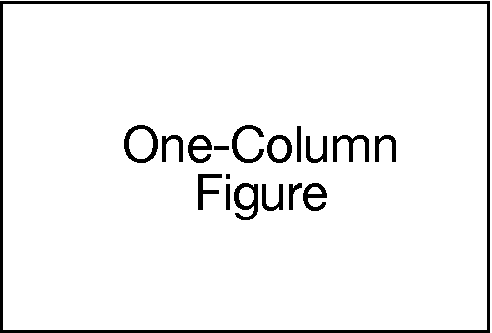
\includegraphics{diagrams/template.pdf}
%%    %
%%    \caption{High-level architecture.}
%%    %
%%    \label{fig:architecture}
%%\end{figure}


\SystemName's future implementation will extend the open source Knative FaaS library.
To facilitate this process, we designed \SystemName-Lite, a simplified proof-of-concept.
There are three core parties involved in \SystemName-Lite:
\begin{enumerate}
	\item \textbf{Function replicas} (e.g., Alice and Bob) that run some application code.
	\item \textbf{Proxy} that manages the function replicas, re-encryption, and load balances requests.
	\item \textbf{Sender} that sends requests to the function, through the proxy.
\end{enumerate}

In previous research, each function replica in a FaaS system would attest to a trusted key
server to obtain a shared key pair.
%
To eliminate this central, trusted dependency, \SystemName
uses decentralized key management with proxy re-encryption.
%
\begin{figure}
    \centering
    \includegraphics[page = 4, width=0.48\textwidth]{diagrams/slides.pdf}
    %
    \caption{\SystemName architecture.}
    %
    \label{fig:arch}
\end{figure}
%
As Figure~\ref{fig:arch} illustrates, the first instance of a given function
generates a key pair and registers the public key in this untrusted registry, managed by the proxy.
Since no private keys or other sensitive information are stored here, this upholds the threat model of an untrusted proxy.
In the future, instances will also register an attestation report that verifies the key was generated in a Trusted Execution Environment\@.
For now, the proxy generates public parameters that are sent to the instances to generate their key pairs.
Since this key generation is done without a TEE in \SystemName-Lite, a malicious cloud provider could obtain access to all function inputs by reading the private key from memory.
\SystemName-Lite does not uphold the same threat model as \SystemName, but we lay the groundwork for future guarantees.

After functions are running and registered with the proxy, the sender can make a request to the function.
The sender must encrypt the message under the public key of just one function instance, despite the potential for any replica to operate on the request.
Therefore, the proxy maintains a record of which instance is the "leader" instance for each function.
They advertise the public keys for those leader instances, and the sender encrypts their message under the public key of the leader for the function they're calling.

When the request gets to the proxy, the proxy will first check if the leader instance is available to handle the request.
If so, the proxy forwards the request to that instance, which can decrypt it with its private key.
If the leader instance is unavailable, the proxy will select an available replica to handle the request.
The proxy will then request the leader instance to generate a re-encryption key from itself to the selected replica.
Upon receiving the key, the proxy will re-encrypt the request to the selected replica, and forward it to that replica.
The selected replica can then decrypt the request with its own private key, and process it.

An interesting aspect of proxy re-encryption is that decrypting an encrypted message and decrypting a re-encrypted message require different decryption method.
This means the decryption performed by the leader is different than the decryption performed by the replica, so
replicas need to be aware of the whether the message is re-encrypted, to call the correct subroutine.

After the message is decrypted, the replica can process the request and send a response back to the proxy, who forwards it to the sender.
In \SystemName-Lite, the function code simply turns the string message uppercase, and sends it back unencrypted.
In the eventual Knative implementation of \SystemName, the replica will encrypt the response back to the sender, or to the next function in the chain, depending on the details of the request.

%As shown in Figure~\ref{fig:arch},
%the first instance of a function generates a key pair and registers the
%public key in an untrusted registry with an attestation report from an Oak
%TEE\@.
%attestation report that verifies the key was generated in an Oak TEE\@.
%
%% When a new replica is launched, the replica registers its own public key,
%% prompting the original instance to generate a re-encryption key.
%
%This enables any instance to encrypt messages for the original key pair,
%allowing independent scaling.
%
%% As a result, each function can encrypt messages for the original downstream
%%% instance's public key, remaining independent of that function's scaling.



%% \textbf{Compilers project proposal}

%% In this section we'll overview the design of the \SystemName system.
%%%
%%First, in section \ref{sec:samba}, I'll describe the proposed \SystemName design.
%%%
%%Then, in section \ref{sec:optimization_design} we'll discuss proposed compiler optimization and general optimizations for the \SystemName system. Finally, in section \ref{sec:eval} we'll cover the means by which I'll evaluate the relative success (or failure) of those performance improvements.
%%%
%% \SystemName applies proxy re-encryption to Function as a Service (FaaS) applications.
%% %
%% We implement it as an extension to Knative Serving\footnote{\url{https://knative.dev/docs/serving/}}, an open-source cloud technology that can function as a FaaS orchestrator.
%% %
%% Knative Serving is a Kubernetes-based platform that enables developers to deploy and manage serverless applications.
%% %
%% Using their existing Knative Serving infrastructure, we can add \SystemName's proxy re-encryption capabilities to functions deployed on Knative.
%% %
%% Knative functions have \texttt{QueueProxy} sidecar containers that can be used to perform instance-level re-encryption operations on the function's behalf.
%% 


%% We implement \SystemName-Lite, a simplified proof-of-concept for the proxy re-encryption scheme applied to FaaS.
%% %
%% To understand how \SystemName-Lite works, I'll describe a simple example where we have a function with a maximum of two replicas, Alice and Bob.
%% For the sake of consistency we'll call the FaaS provider/orchestrator Proxy.
%% For simplicity in this explanation, we'll assume not only Proxy, but also Alice and Bob are always running, which defeats the entire purpose of FaaS, but doesn't effect our analysis of the cryptographic operations.
%% We assume that Alice's public key will be known by any prospective clients wishing to run the function, since she is the leader replica, so Proxy will advertise her public key as the public key of the function.
%% Requests destined for the function are encrypted under Alice's public key, and sent by some Sender to Proxy.
%% Proxy then load balances, determining if Alice can currently accept a request.
%% If so, Proxy forwards the request to Alice, who can decrypt it with her private key, and send her response to the Proxy, who forwards it to Sender.
%% If not, Proxy selects an availible replica, in this case Bob, and requests a re-encryption key from Alice to Bob (if one hasn't already been made).
%% Proxy then re-encrypts the request to Bob, forwards the request to Bob.
%% Bob decrypts, and responds to Proxy, who forwards that response to Sender.
%% The decryption operation for a re-encrypted message is different than a normal RSA decryption, which we'll touch on more in section~\ref{sec:PRE}.

%% \subsection{Optimization}
%% \label{sec:optimization_design}
%% 
%% The performance impact of adding proxy re-encryption to an otherwise un-encrypted program is no secret.
%% The AFGH authors aren't shy about this, but do mention that if they had gone to greater lengths to select proper compiler optimizations, these effects could be reduced.
%% \cite{afgh}
%% That is the motivation for this proposal.
%% With our proxy re-encryption implementation written in Go, we have access to a compiler with many optimizations already built in, and a rich ecosystem of open source extensions.
%% The primary contribution of this project will be, through theoretical research, as well as trial and error, determining what set of optimizations for the Go compiler produce the best results for proxy re-encryption in the Samba system.
%% 
%% Beyond the possible compiler optimizations, we will make sure to do another simple optimization at the code level.
%% If we were to write the least amount of code possible to implement proxy re-encryption within Samba, that would probably involve the initial replica generating re-encryption keys to re-encrypt messages to itself, so we wouldn't have to code anything for that "base case."
%% The optimization here would be to simply code specifically for the case where the request is load balanced to the initial replica, and skip the re-encryption key generation, and re-encryption steps.
%% This will limit the cryptographic operations performed to those that are absolutely necessary.
%% 
%% \subsection{Evaluation}
%% \label{sec:eval}
%% 
%% Knative and the Samba extension are both written in Go.
%% Among the many benefits of the Go Programming Language is its standard library, which contains many idiomatically written packages for tasks developers need to perform frequently.
%% In our case, we'll make extensive use of the "testing" package, and specifically its benchmarking support.
%% This will be most helpful for testing the effectiveness of our optimizations on the \texttt{alice}, \texttt{bob}, and \texttt{proxy} binaries within the proof-of-concept \SystemName-Lite portion of the project.
%% 
%% Additionally, Knative itself offers a number of ways to benchmark components in its distributed system.
%% \cite{knative_serving}
%% We will use these tests to compare the performance of Knative's Autoscaling Sample App without the Samba extension vs. with the Samba extension.
%% \cite{autoscale_sample_app_go}


%%
%In previous research, to ensure each function replica used the same key pair,
%each replica would attest to a trusted key server, which then provided the
%correct key pair based on the replica's attestation measurement.
%%
%To remove this reliance on centralized, trusted infrastructure, \SystemName
%employs a decentralized key management system using proxy re-encryption.
%%
%\begin{wrapfigure}{l}{0.5\textwidth}
%    \centering
%    \includegraphics[page = 4, width=0.48\textwidth]{diagrams/slides.pdf}
%    %
%    \caption{\SystemName architecture.}
%    %
%    \label{fig:arch}
%\end{wrapfigure}
%%
%As Figure~\ref{fig:arch} illustrates, the initial instance of the function
%generates a key pair and registers the public key in an untrusted registry,
%along with an attestation report that verifies the key was generated in an Oak
%TEE\@.
%%
%When the FaaS platform launches a new replica of the function, the replica
%generates and registers its own public key.
%%
%This triggers the FaaS platform to request the initial function instance to
%produce a re-encryption key for the new replica.
%%
%As a result, each function can encrypt messages for the original instance’s
%public key, remaining independent of the function's scaling.



%%\begin{table}[t!]
%%    \small
%%    \caption{Time (s) to Re-encrypt a Bucket of Size 1G}
%%    \label{tab:enclave-overhead}
%%    \centering
%%    \begin{tabular*}{0.48\textwidth}{|r|@{\extracolsep{\fill}}r|r|}
%%        \hline
%%        \textbf{Environment}  &\textbf{Akeso}  &\textbf{Strawman}  \\
%%        \hline
%%        \textbf{Confidential VM}    &47.231  	 &118.239  \\             
%%        \textbf{Non Confidential VM}        &44.907	    &109.366 \\            
%%        \hline 
%%    \end{tabular*}
%%\end{table}

%% \textbf{adwait}
%% 
%% There are a number of open source projects for various parts of the project that we will be extending.
%% 
%% \subsection{Function Runtime}
%% We performed all development and testing on an AMD-SEV SNP machine, to later take advantage of Trusted Execution Environment features.
%% We have not yet enabled these features in the course of development.
%% We ported an open source proxy re-encryption library from C to Rust in order to be callable from within the later boot stages of the Oak Restricted Kernel.
%% The kernel extension itself is still a work in progress.
%% There is a lot to sort through to determine where exactly in the boot stages would be the best place to perform re-encryption and decryption
%% to be able to work with the data.
%% 
%% \subsection{FaaS Orchestration}
%% Function as a Service paradigms are implemented differently by different platforms.
%% Amazon Lambda, Google Cloud Functions, and Azure Functions are all well-known and closed source, all with (presumably) completely different architectures.
%% 
%% The open source FaaS landscape is no more homogenous than its corporate counterpart.
%% Additionally, some are partially open source, with certain paywalled features, and others use deprecated dependencies which makes setup a non-trivial problem.
%% This was a major hurdle for development, and battling the idiosyncracies of these FaaS frameworks accounts for much of the progress (or lack thereof) made on this project.
%% 
%% \subsubsection{Firecracker}
%% Firecracker is partially open source, and disbatches requests to networks of MicroVMs.
%% Since it doesn't support custom kernels out of the box, and a lot of the code is written with MicroVM specific APIs, extending this project to accomodate the Oak Restricted Kernel for SAMBA would amount to basically a full rewrite.
%% 
%% \subsubsection{OpenFaaS}
%% OpenFaaS, perhaps misleadingly, is not fully open source.
%% Components such as the load balancer that creates function replicas are only availible as binaries, and therefore the modifications that we need to make are not possible with OpenFaaS.
%% 
%% \subsubsection{OpenWhisk}
%% OpenWhisk is fully open source, and is used in a variety of recent papers. That said, the repository seems barely maintained in 2024, and older versions of Java (Java 8), Docker, and Ubuntu may be required to cohesiveliy run it.
%% Investigations to that effect are another significant contributor to delay in this project.
%% We anticipate continuing efforts, potentially of a known working fork from a researcher who has used OpenWhisk successfully in recent years.
%% Also, I will re-double my efforts following and modifying few-yearold open source documentation to get development up and running, by emulating all dependencies as closely as possible.
%% 
%% \subsubsection{Open Function}
%% Open Function is another open source function orchestrator, which we will look into as an implementation option.
%% 

\section{Implementation}
\label{sec:implementation}

Congue malesuada turpis taciti, condimentum erat eget gravida est. Mollis eu
maximus sagittis cras lectus massa nam primis. Porta quis magnis et etiam
maecenas odio. Lacus ad a eleifend imperdiet cubilia auctor tristique montes.
Fringilla facilisi diam hendrerit ut purus. Neque mus feugiat sodales luctus at
rutrum class sed venenatis. Massa tortor facilisis ultrices vehicula dui
sodales.

Morbi nisi class sit ante taciti rutrum magna. Per faucibus litora justo velit
nibh orci scelerisque lobortis feugiat. Sed tincidunt lacus placerat quisque
rhoncus. Lectus turpis placerat metus parturient tempor tortor condimentum
dapibus. Id dui habitasse lorem sapien in eu maximus. Pellentesque vulputate
nibh orci ut consectetur praesent.

Nisi quam pellentesque proin blandit sollicitudin himenaeos facilisis cubilia
fringilla. Aliquam conubia faucibus non auctor turpis libero sapien aliquam.
Maximus imperdiet aliquam nostra eget condimentum augue ut nam finibus? Quisque
ligula orci habitasse porttitor mauris senectus ex feugiat. Varius nisl
suspendisse metus finibus proin ridiculus ipsum; ex curabitur? Dictumst nulla
vitae quam pulvinar feugiat odio eu sapien tempor. Quis montes donec laoreet
rutrum vel nam duis mattis. Turpis ut congue elit dis, leo litora aliquet
metus?

\begin{figure}[t]
    \centering
    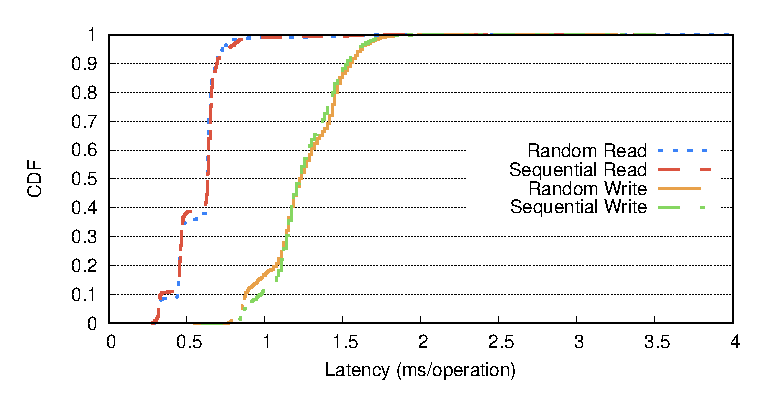
\includegraphics[width=0.5\textwidth]{figs/latency-cdf}
    %
    \caption{CDF of latencies for object read and write operations with \System (object size = 10M).}
    %
    \label{fig:latency-cdf}
\end{figure}

\section{Evaluation}
\label{sec:evaluation}

%% \begin{figure*}
%%     \centering
%%     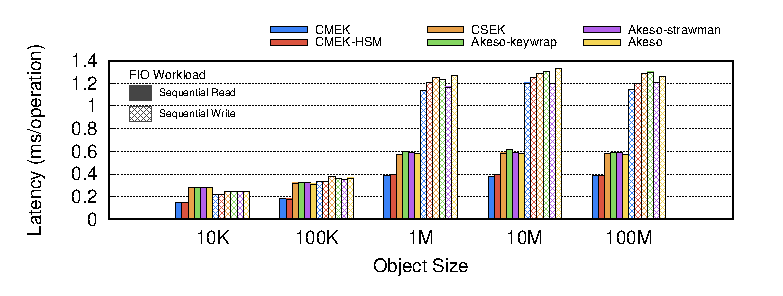
\includegraphics[width=\textwidth]{figs/fsop-latency-hist-2col}
%%     %
%%     \caption{Latency of read and write operations for encrypted cloud storage.}
%%     %
%%     \label{fig:fsop-latency-hist-2col}
%% \end{figure*}

To evaluate the performance of the \SystemName library, we wrote a series of benchmark tests.
Not only did we test the performance of \SystemName using proxy re-encryption, but we also compared it to an RSA implementation.
Note that actually implementing \SystemName with RSA instead of PRE would defeat the purpose, as either the proxy would have to be trusted with every instance's private key, or all instances of the same function would have to share the same key pair.

For the RSA implementation, we only benchmarked the functions responsible for encrypting and decrypting messages, since "re-encryption" is not a concept in RSA.
For the proxy re-encryption implementation, we benchmarked the \SystemName functions responsible for encrypting and decrypting messages, generating re-encryption keys, and re-encrypting messages.
Additionally, we benchmarked the underlying proxy re-encryption functions, from the PRE package we wrote.
The benchmarks were run using the Go testing framework, which provides a simple way to measure the time taken by each function.
Our results from an 8-core M1 Mac of for the \SystemName benchmarks are shown in Figure~\ref{fig:samba-bench}, and the PRE benchmarks are shown in Figure~\ref{fig:pre-bench}.

\begin{figure}
	\centering
	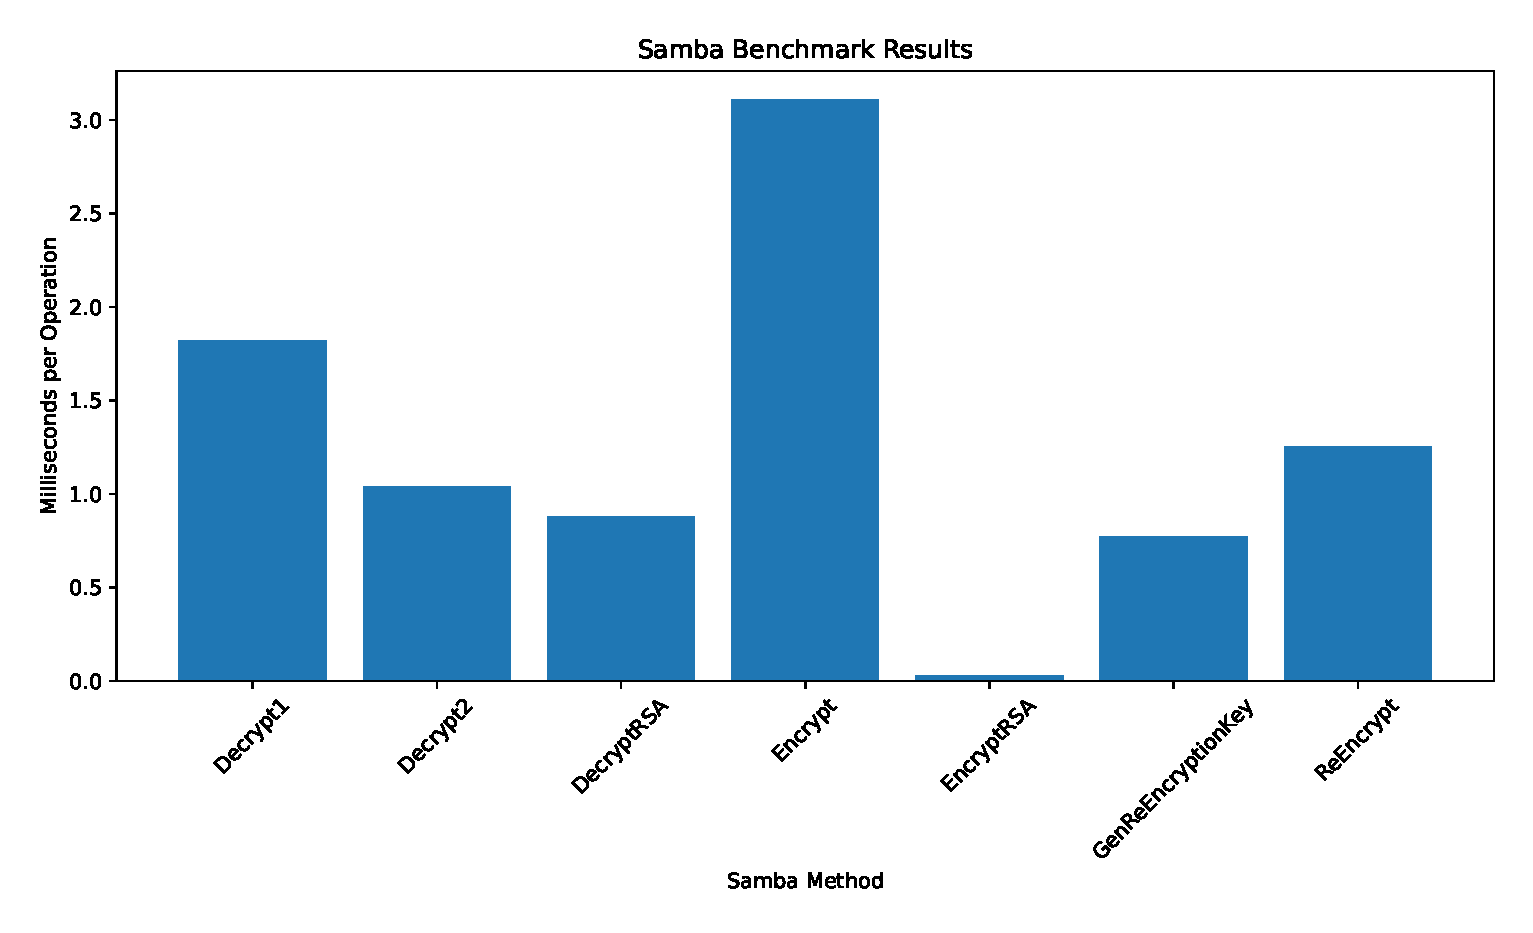
\includegraphics[width=0.48\textwidth]{figs/samba-bench}
	%
	\caption{Benchmark results for the \SystemName library, with both PRE and RSA operations.}
	%
	\label{fig:samba-bench}
\end{figure}

\begin{figure}
	\centering
	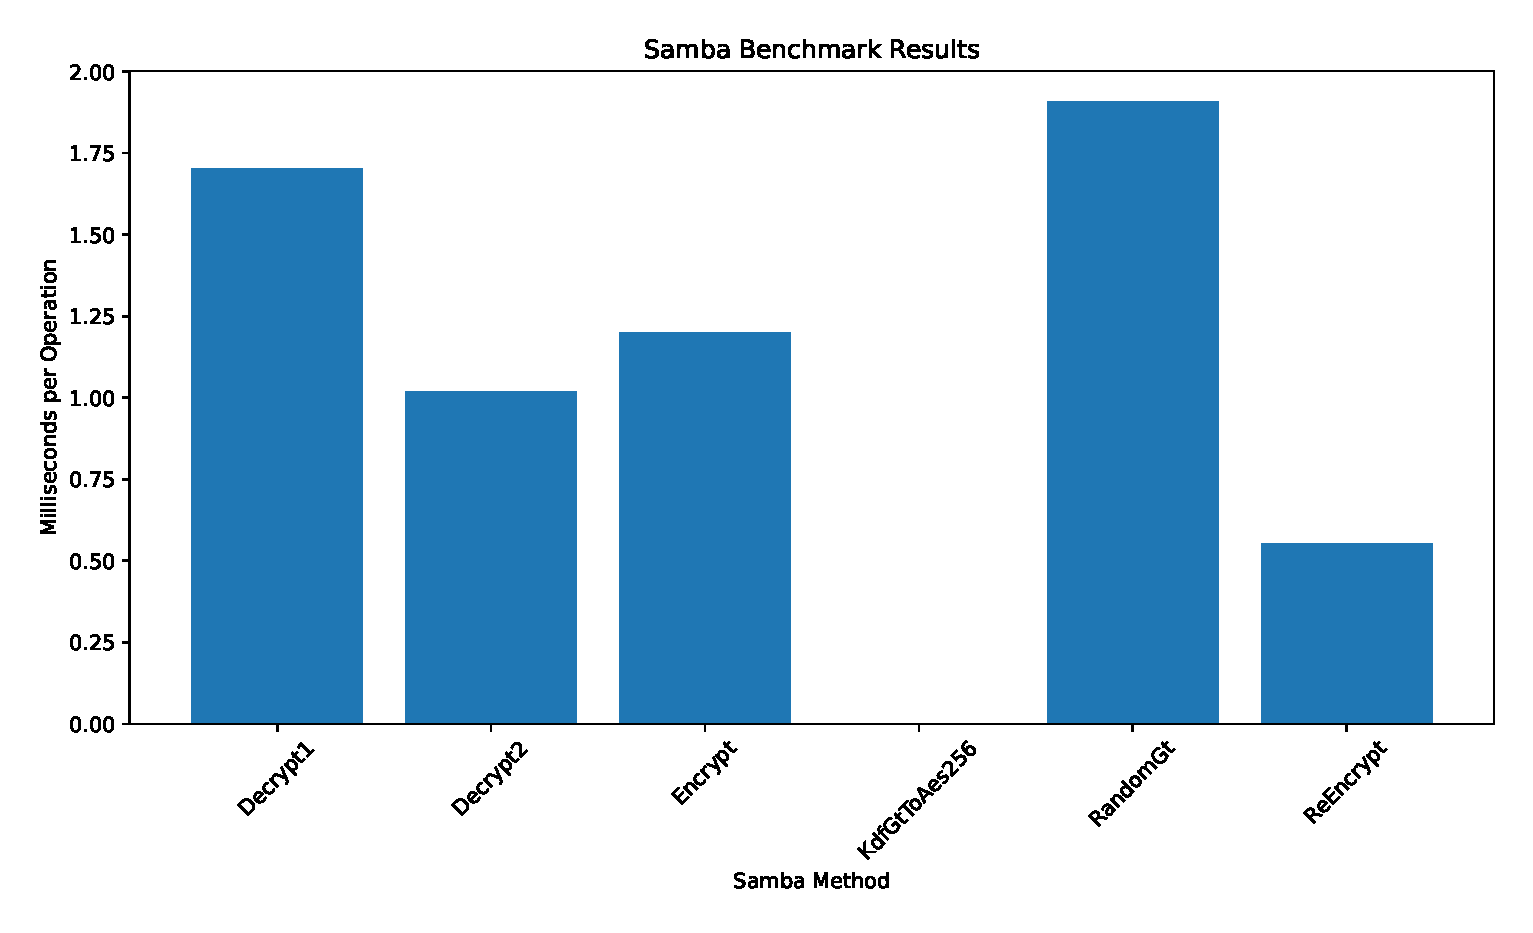
\includegraphics[width=0.48\textwidth]{figs/pre-bench}
	%
	\caption{Benchmark results for the PRE library.}
	%
	\label{fig:pre-bench}
\end{figure}



%% The encryption performed by the external sender is the least expensive, which is good for responsiveness, since the user's request will be on its way relatively fast.
%% The generation of a re-encryption key and the use to that key to re-encrypt are more expensive.
%% Interestingly, the decryption of a re-encrypted message takes about twice as long as the decryption of a message encrypted under the original RSA.
%% 
%% To compare \SystemName's efficiency relative to cryptographic alternatives, we wrote functions and microbenchmarks for simple RSA, where we assume that either only one replica can exist for each function, or the proxy is trusted, and uses the leader's private key to decrypt and re-encrypt messages to the various replicas.
%% The benchmark results for RSA are shown below.

%% \color{red}
%% show RSA results
%% 
%% Compare the two
%% 
%% Show some figures
%% 
%% Justify the increased overhead
%% \color{black}


%
%% We will assess \SystemName's performance by measuring its overhead on
%% open-source AWS Lambda serverless applications, such as
%% CodePipeline\footnote{\url{https://github.com/aws-samples/aws-codepipeline-stepfunctions}}
%% and
%% MapReduce\footnote{\url{https://github.com/awslabs/lambda-refarch-mapreduce}},
%% which differ in chain length and complexity.
%% %
%% To decompose the overheads, we will compare \SystemName with: \emph{(1)}
%% \SystemName-strawman, which provides each function replica with the same key
%% pair via an enclaved key service; \emph{(2)} \SystemName-untrusted, which runs
%% functions in a non-confidential Oak VM; and \emph{(3)} standard OpenFaaS, using
%% OpenFaaS's default function runtime.
%% %
%% We will utilize the \texttt{wrk}\footnote{\url{https://github.com/wg/wrk}} and
%% Grafana \texttt{k6}\footnote{\url{https://grafana.com/oss/k6/}} benchmarking
%% tools to measure end-to-end latency, cold start times, and scalability.



%% \textbf{adwait}
%% 
%% % Evaluation (don't forget to interpret your data)
%% As no evaluation has taken place yet, I will lay out the steps by which we will likely evaluate the completed system. 
%% 
%% We will evaluate both the performance and cost of SAMBA, by answering the following research questions:
%% 
%% \newrq{rq:confidentiality}{How well does Samba ensure data confidentiality across functions without relying on centralized key management?}
%% 
%% \newrq{rq:control_flow_integrity}{How does Samba guarantee control flow integrity across function chains without a global controller?}
%% 
%% \newrq{rq:performance}{What is the performance overhead introduced by Samba's cryptographic protocols (proxy re-encryption and aggregate signatures) compared to unsecured FaaS usage, and comparable secure solutions?}
%% 
%% \newrq{rq:scalability}{How do Samba's decentralized key management system and aggregate signatures scale with large function graphs?}
%% 
%% To answer these research questions, we will design and implement Samba as an extension of Project Oak's Restricted Kernel.
%% We will evaluate Samba's security claims using some simple custom function-chain applications, and several real-world AWS-based applications (e.g., HelloRetail, CodePipeline, MapReduce).
%% 
%% \rqref{rq:confidentiality}
%% will be evaluated by simulating adversarial attempts from cloud providers to access encrypted inputs/outputs by running Samba in a VM on a "malicious" operating system.
%% \rqref{rq:control_flow_integrity}
%% will be evaluated by inserting malicious functions into a Samba chain and verifying whether deviations from the expected flow are detected and handled.
%% \rqref{rq:performance} and \rqref{rq:scalability}
%% will be measured using load-testing tools like \texttt{wrk} and \texttt{Grafana k6}, measuring end-to-end latency, cold start times, and autoscaling effectiveness, and comparing different Samba implementations with standard FaaS implementations.
%% 
%% \subsection{Confidentiality Evaluation}
%% We hypothesize that Samba doesn't leak any information to a malicious operating system.
%% This addresses \rqref{rq:confidentiality}.
%% We will deploy a chain of custom functions in Samba that runs properly, with all hardware and software described earlier.
%% Then, we will make attempts through the OS to read data from one of the Samba functions.
%% This simulates the case of an adversarial cloud provider.
%% We expect that no data will leak from within Samba to the OS. Success is defined as: All attempts by the OS to read data from within Samba fail.
%% 
%% \subsection{Control Flow Integrity Evaluation}
%% We hypothesize that Samba can detect and prevent unauthorized modification of data between functions in a graph, and unauthorized reordering of functions.
%% This addresses \rqref{rq:control_flow_integrity}.
%% We will deploy a chain of custom functions in Samba that runs properly, with all hardware and software described earlier.
%% Then, we'll reroute the ouput and input of two adjacent functions, respectively, to a "malicious" function, running on a non-TEE-based linux VM.
%% This simulates a man-in-the-middle scenario, where in insecure chains an adversary could read or change data.
%% We expect that no unauthorized party can reorder functions or modify data. Success is defined as:
%% \begin{enumerate}
%%     \item The function recieving input from the malicious function detects the invalid signature, throws an error, and ends execution.
%%     \item The malicious function is unable to decrypt any of the input it recieves from the previous function.
%% \end{enumerate}
%% 
%% \subsection{Cost Evaluation}
%% We hypotesize that we can provide the security guarantees of Samba with minimal performance overhead compared to standard FaaS platforms.
%% This addresses \rqref{rq:performance} and \rqref{rq:scalability}.
%% We will deploy several open-source AWS Lambda- and AWS Step-based FaaS applications, like HelloRetail, CodePipeline, and MapReduce.
%% We'll compare the performance our full Samba implementation with
%% \begin{enumerate}
%% \item a Samba implementation without proxy re-encryption, simply using a key service to provide each function with the same key pair,
%% \item a Samba implementation run on an unconfidential VM (no TEE), and
%% \item a standard OpenFaaS VM, with a standard runtime.
%% \end{enumerate}
%% We'll use wrk and Grafana to compare the performance.
%% We'll measure end-to-end latency, cold start times, and autoscaling behavior for our different environments.
%% Success is defined as maintaining minimal performance overhead (perhaps 10\%) compared to standard FaaS environments.

\section{Related Works}
\label{sec:related}

Tortor tristique praesent mus mollis vestibulum arcu dolor. Lacinia vel metus
semper, ultricies eleifend rhoncus eleifend. Leo dictum fusce molestie gravida
hac dui consectetur etiam. Aquam vel cubilia tellus dui sed porta rhoncus id.
Maecenas pharetra hac bibendum cursus montes. Id in phasellus felis habitant
habitant fermentum accumsan dis dapibus. Ipsum curae dictumst leo eget massa
quis vestibulum ac lacus. Fermentum class vulputate a id egestas aliquam id.
Vel bibendum ac nascetur class leo molestie natoque a.

\section{Conclusion}
\label{sec:conclusion}

% https://queue.acm.org/detail.cfm?id=3623461
As Mark Russinovich, CTO of Microsoft Azure, famously stated, in the future,
``confidential computing will just be
computing''~\cite{23-acm_queue-confidential_computing}.
%
Realizing this vision requires rethinking today's software systems to make
confidential computing practical and accessible.
%
This thesis takes a first step by bringing confidentiality to a widely used
model---Function as a Service---while maintaining compatibility with existing
applications through our system, \SystemName.
%
\SystemName demonstrates that trusted hardware alone is not enough to satisfy
the complex requirements of modern software systems.
%
Instead, combining trusted hardware with cryptographic
techniques---specifically, proxy re-encryption in \SystemName's case---enables
secure and scalable solutions.
%
To support future work, we have made our \SystemName-lite implementation
publicly available at \url{https://github.com/etclab/samba}, along with our
proxy re-encryption library at \url{https://github.com/etclab/pre}.




%% \textbf{adwait}
% Conclusions (don't summarize your work here. That's what the abstract
% was for. Instead provide some philosophical ruminations of your work and
% future possibilities, i.e., conclusions that you have arrived at as a
% result of your work.)




%%%%%%%%%%%%%%%%%%%%%%%%%%%%%%%%%%%%%%%%%%%%%%%%%%%%%%%%%%%%%%%%%%%%%%%%%%%%

\bibliographystyle{ACM-Reference-Format}
\bibliography{conferences,refs}

\end{document}
\endinput
%%
%% End of file `sample-sigconf.tex'.
